\documentclass[9pt,twocolumn,twoside]{pnas-new}
% Use the lineno option to display guide line numbers if required.
% Note that the use of elements such as single-column equations
% may affect the guide line number alignment.

% new commands:
\newcommand{\cel}{\emph{C.~elegans}}
\newcommand{\dicty}{\emph{D.~discoideum}}
\newcommand{\egl}{\emph{egl-9}}
\newcommand{\rhy}{\emph{rhy-1}}
\newcommand{\vhl}{\emph{vhl-1}}
\newcommand{\eglvhl}{\emph{egl-9;vhl-1}}
\newcommand{\eglhif}{\emph{egl-9;hif-1}}
\newcommand{\hif}{\emph{hif-1}}
\newcommand{\fog}{\emph{fog-2}}
\newcommand{\nhr}{\emph{nhr-57}}
\newcommand{\ecol}{\emph{E.~coli}}

\newcommand{\egln}{1959}
\newcommand{\rhyn}{2650}
\newcommand{\vhln}{1039}
\newcommand{\eglvhln}{3330}
\newcommand{\hifn}{1026}
\newcommand{\eglhifn}{381}
\newcommand{\fogn}{}

\newcommand{\egltargets}{}
\newcommand{\rhytargets}{}
\newcommand{\vhltargets}{}
\newcommand{\hiftargets}{}
\newcommand{\hifhydroxytargets}{}


\templatetype{pnasresearcharticle}[9pt,twocolumn,twoside,lineno] % Choose template
% {pnasresearcharticle} = Template for a two-column research article
% {pnasmathematics} = Template for a one-column mathematics article
% {pnasinvited} = Template for a PNAS invited submission

\title{Genetic Analysis of a Metazoan Pathway using Transcriptomic Phenotypes}

% Use letters for affiliations, numbers to show equal authorship (if applicable) and to indicate the corresponding author
\author[a,b]{David Angeles-Albores}
\author[a,b]{Carmie Puckett Robinson}
\author[a]{Brian Williams}
\author[a]{Igor Antoshechkin}
\author[a,b]{Paul W Sternberg}

\affil[a]{Department of Biology and Biological Engineering, Caltech, Pasadena, USA, 91125}
\affil[b]{Howard Hughes Medical Institute}

% Please give the surname of the lead author for the running footer
\leadauthor{Angeles-Albores}

% Please add here a significance statement to explain the relevance of your work
\significancestatement{Measurements of global gene expression are often used as descriptive tools that identify genes that are downstream a perturbation. In theory, there is no reason why measurements of global transcriptomes could not be used as a quantitative phenotype for genetic analysis. Here, we show that transcriptomes can be used for epistasis analysis in a metazoan, and that transcriptomes afford far more information per experiment than classic genetic analysis. By using transcriptomes as quantitative phenotypes, we can accurately predict interactions between genes, while at the same time identifying genes common to a pathway.
When pathways branch, it is also possible to identify gene batteries that are associated with each end of the branch point. Finally, genes that would result in invisible visible phenotypes in an animal are not likely to be invisible at the transcriptome phenotype due to the exquisite granularity present in these structures, which represents an important advance towards studying small effect genes that make up the majority of animals' genetic repertoire.}

% Please include corresponding author, author contribution and author declaration information
\authorcontributions{DA and PWS wrote the manuscript. CPR performed all experiments. BW performed library preparation. IA performed sequencing. DA performed all analysis and blinded genetic reconstruction.}
\authordeclaration{The authors declare no conflict of interest.}
% \equalauthors{\textsuperscript{1}A.O.(Author One) and A.T. (Author Two) contributed equally to this work (remove if not applicable).}
\correspondingauthor{\textsuperscript{2}To whom correspondence should be addressed. E-mail: pws@caltech.edu}

% Keywords are not mandatory, but authors are strongly encouraged to provide them. If provided, please include two to five keywords, separated by the pipe symbol, e.g:
\keywords{genetics $|$ RNA-seq $|$ \cel{} $|$ hypoxia $|$ transcriptomics}

\begin{abstract}
RNA-seq is a technology that is commonly used to identify genetic modules that are responsive to a perturbation. In theory, global gene expression could also be used as a phenotype, with all the implications that has for genetic analysis. To that end, we sequenced four single mutants and two double mutants of the hypoxia pathway in \cel{}. We successfully analyzed the single mutants in a blinded fashion to predict the genetic relationships between the genes, and used the double mutants as a test of our predictions and to infer the directionality of the relationship. We show that genes along a pathway tend to decorrelate as a result of alternative regulatory modes and crosstalk with other pathways; and that this decorrelation accurately reflects functional distance between genes. As a by-product of our analysis, we identified a core set of XXX genes that are involved in the \hif{}-dependent hypoxia response in the worm.\end{abstract}

\dates{This manuscript was compiled on \today}
\doi{\url{www.pnas.org/cgi/doi/10.1073/pnas.XXXXXXXXXX}}

\begin{document}

% Optional adjustment to line up main text (after abstract) of first page with line numbers, when using both lineno and twocolumn options.
% You should only change this length when you've finalised the article contents.
\verticaladjustment{-2pt}

\maketitle
\thispagestyle{firststyle}
\ifthenelse{\boolean{shortarticle}}{\ifthenelse{\boolean{singlecolumn}}{\abscontentformatted}{\abscontent}}{}

% If your first paragraph (i.e. with the \dropcap) contains a list environment (quote, quotation, theorem, definition, enumerate, itemize...), the line after the list may have some extra indentation. If this is the case, add \parshape=0 to the end of the list environment.
\dropcap{B}y definition, phenotypes are measurable traits that are related to genotypes via a formal mapping function. In order to infer a genetic relationship, two genes must act on the same phenotype. However, the converse, that two genes share a phenotype, does not imply that these genes interact. In order to demonstrate an interaction, a geneticist must show that a double mutant exhibits sign epistasis. The phenotype of the single and double mutants combined then provides enough information to infer the genetic relationship between them, and in some cases it can also be sufficient to infer order.

Previous work in \dicty{} has shown that transcriptomes contain sufficient information to infer genetic relationships in a simple eukaryote~\cite{}. This early work was performed using microarray technology, which suffered from drawbacks related to sensitivity. New technologies such as RNA-seq~\cite{} do not suffer from these drawbacks. Developments in the area of transcriptomics have also made important progress towards cheaper sequencing~\cite{}, better read alignment~\cite{} and differential analysis~\cite{}.
As a result, RNA-seq has been used to identify key regulatory modules involved in a variety of processes, inncluding T-cell regulation~\cite{} or planarian stem cell identification~\cite{}. However, even in these novel applications, transcriptomes largely serve a descriptive role, and are important for hypothesis generation and target acquisition as opposed to hypothesis testing and model creation.
Here, we show that transcriptomes contain extremely strong, robust signals that can be used to infer relationships between genes in complex metazoans by reconstructing a known pathway, the hypoxia pathway in \cel{} using RNA-seq in a blinded manner. We show that various techniques, including pairwise comparisons, clustering or \emph{in silico} qPCR can be used to generate a testable model of genetic interactions. A complete, interactive version of the analysis is also available at URL.

\section*{Results}
\subsection{Clustering visualizes epistatic relationships between genes}
\label{sub:Clustering}

Clustering is a well-known technique in bioinformatics to identify relationships between data~\cite{}. As a first step in our analysis, we wanted to make sure that clustering by Transcripts Per Million (TPM) yielded genetically relevant information. Indeed, when blind, unsupervised clustering was performed on the data, three clusters emerged naturally. \hif{} and \egl{};\hif{} clustered along with the wild-type; whereas \egl{}, \egl{};\vhl{}, \vhl{} and \rhy{} all clustered away from the wild-type. Finally, our negative control \fog{} was in its own cluster (see Fig.~\ref{fig:dendrogram}). These clusters make intuitive biological sense:
\hif{} does not have a large role in normoxic circumstances, and is continuously degraded in a normal environment~\cite{}. As a result, \hif{} exists only at low levels in a normoxic worm. This strong control on the protein levels of \hif{} is known to be mediated by a pathway involving \egl{}, \vhl{} and \rhy{}\cite{}. Whereas the \hif{} is largely wildtype in normoxic environments, genes that control \hif{} expression have visible phenotypes. The expectation that \hif{} should therefore cluster near the wild-type and the control genes should cluster away from the wild-type are therefore realized. Moreover, unsupervised clustering correctly identified epistatic relationships in double mutants: the \hif{};\egl{} double mutant clustered with the wild-type (this double mutant no longer has an \emph{egl} phenotype), and the \egl{};\vhl{} mutant clusters with the \egl{} and \vhl{} single mutants.
Thus, we conclude that expression data contains enough signal to cluster genes in a meaningful manner.

% dendrogram
\begin{figure}%[tbhp]
\centering
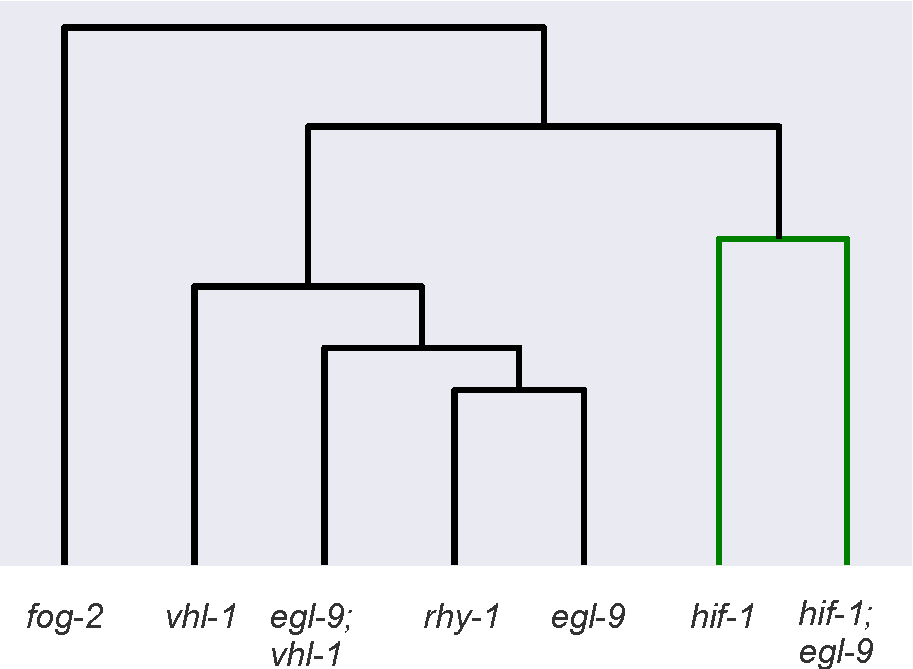
\includegraphics[width=.8\linewidth]{figs/dendrogram.pdf}
\caption{Blind unsupervised clustering of various \cel{} mutants. Genes cluster in a manner that is biologically intuitive. Genes that have visible phenotypes under normoxia cluster away from the wild-type, and when these genes act in the same pathway, they cluster together (i.e, \egl{}, \vhl{}, and \rhy{}). Genes that look wild-type under normoxia cluster near the wild-type..}
\label{fig:dendrogram}
\end{figure}

\subsection{Transcriptomic correlations can predict genetic regulation}
\label{sub:Transcriptomic genetic analyses}

Theoretically, two genes that have a linear positive interaction should be positively correlated in their overlapping transcriptomes, whereas two genes that have a linear negative interaction should be negatively correlated in their transcriptomes. Formally, if we consider that a gene \emph{A} has a transcriptome \emph{\{A\}} associated with it, and if we consider a second gene \emph{B} with an associated transcriptome \emph{\{B\}} that is activated by \emph{A} (that is, $B \in \{A\}$, such that $\{B\} \subset \{A\}$), then it follows that genetic knockout of \emph{A} or \emph{B} should both lead to the same perturbation of the transcriptome \emph{\{B\}}.
Therefore, it follows that two genes should be strongly positively correlated in the overlap between their transcriptomes if they have positive regulatory associations. Conversely, it follows that if two mutants have overlapping transcriptomes, and if these transcriptomes have a strong positive association, it is likely that these two genes share a positive regulatory association. In other words, transcriptomic correlation is a good predictor of genetic regulation.

Although transcriptomic correlations could theoretically be used for the purposes of identifying genetic regulation, noise from measuring 20,000 genes in multiple different genotypes could cause serious interference with any inferences. Additionally, genes sometimes experience multiple modes of regulation, including positive and negative regulation, from the same gene or pathway. If a positive and a negative signal are both present in a transcriptome, running a naive regression will result in a value close to zero.
Therefore, we took steps to mitigate noise in the form of outliers. As a first mitigation attempt, we rank-tranformed the regression coefficients output by Kallisto. This has the effect of mitigating outliers by resetting the difference between adjacent coefficients to unity. Secondly, we performed robust Bayesian regressions using a Student T distribution as a prior. A Student T distribution decays less quickly than a normal distribution, which causes the model to consider outliers to be less informative than traditional frequentist regressions which effectively use a normal prior.

% genetic correlations
\begin{figure}%[tbhp]
\centering
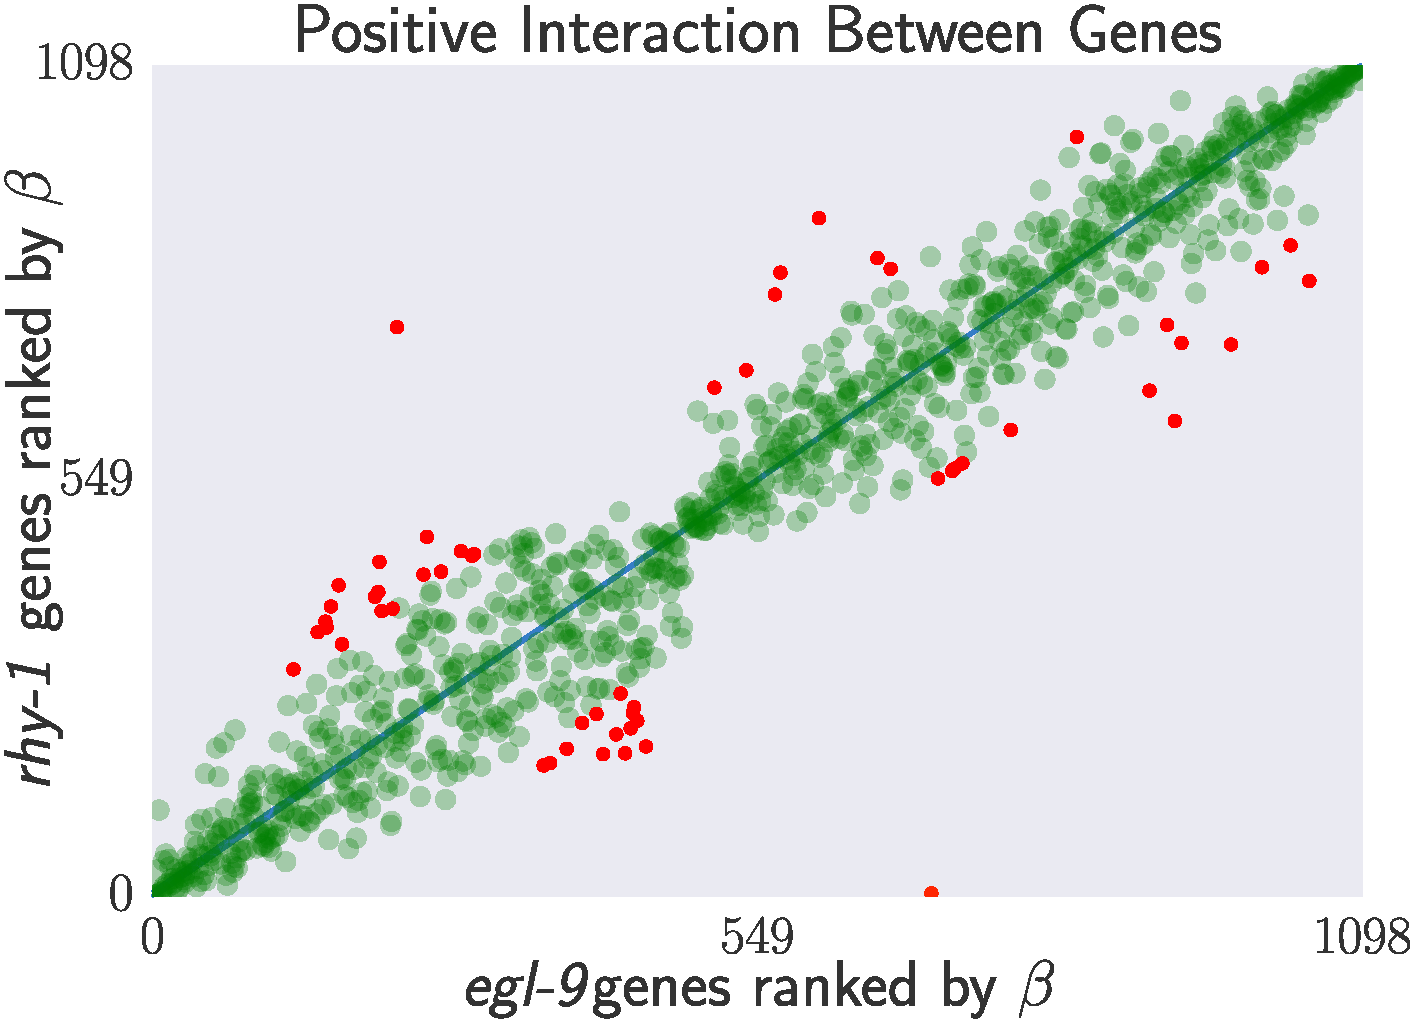
\includegraphics[width=.8\linewidth]{figs/correlative_genetics.pdf}
\caption{\textbf{Top} Schematic Diagram showing that genes that interact positively should have a positive transcriptomic correlation, whereas genes that interact negatively should have a negative correlation. Single genes are referred to by their names (A, B), and the transcriptome associated only with gene X is referred to as \{X\}. We use superscripts to denote expression level. In this case, 0 = no expression (knockout); 1 = WT level; 2 = Greater than WT level.\ \textbf{Bottom} Empirical demonstration that transcriptomes between two interacting genes can be extremely well correlated when genes are ranked by expression changes relative to a wild-type.}
\label{fig:genetic_interactions}
\end{figure}

Having mitigated the effect of outliers, we saw that for certain gene pairs, their transcriptomes correlated very well when genes were ranked by their expression changes (see Fig.~\ref{fig:genetic_interactions}). Having confirmed that we could extract strong signals from these transcriptomes, we proceeded to generate all pairwise correlations between interactomes and we weighted the correlations by the number of genes that participated in the correlation (that were not outliers) divided by the total number of genes detected in all samples.
The regression slopes recapitulated a network with three `modules': A control module, a responder module and an uncorrelated module (see Fig.~\ref{fig:heatmap}). We were able to identify a strong positive interaction between \egl{} and \rhy{}. Part of the reason for this lies in the fact that the transcriptomes for these genes consisted of 1,813 and 2,457 significantly altered genes respectively and the overlap between both genes was quite extensive.
On the other hand, none of the correlations between \hif{} and its controlling genes are negative. On the one hand, we expect that the \hif{} transcriptome is most susceptible to noise because the protein is expressed at low levels in normoxic environments. However, the \hif{} transcriptome consists of 937 differentially expressed genes, and the overlap between \hif{} and all its controlling genes was always greater than 200 genes. Moreover, the unweighted correlation between all the pairwise genes was >0.7 for all comparisons. This means it is unlikely that the positive correlations are purely a result of noise.

In order to rule out noise, we calculated the probability that \hif{} and its regulatory genes are drawing their transcriptomes from a common pool; in other words, the probability that \hif{} and the regulatory genes share an isotranscriptome (we use the word isotranscriptomes to refer to two transcriptomes that have the same set of genes, and where these genes change in the same way relative to a control).
One way to do this is to take, for example, \egl{} or \hif{}, and select whichever transcriptome has a greater number of differentially expressed genes and paint these genes as red balls in an urn, whereas any genes that are not differentially expressed are painted as white balls. Then, we can ask what the probability of selecting $N$ balls in total of which $K$ are red balls is using a hypergeometric function, taking into account that a gene will be red only if it changes in the same way in both transcriptomes. We find that the probability that \hif{} is interacting positively with \egl{}, \rhy{} and \vhl{} is essentially unity. We conclude that under a normoxic environment, \hif{} has a positive genetic association with \egl{}, \rhy{} and \vhl{}.
% heatmap
\begin{figure}[tbhp]
\centering
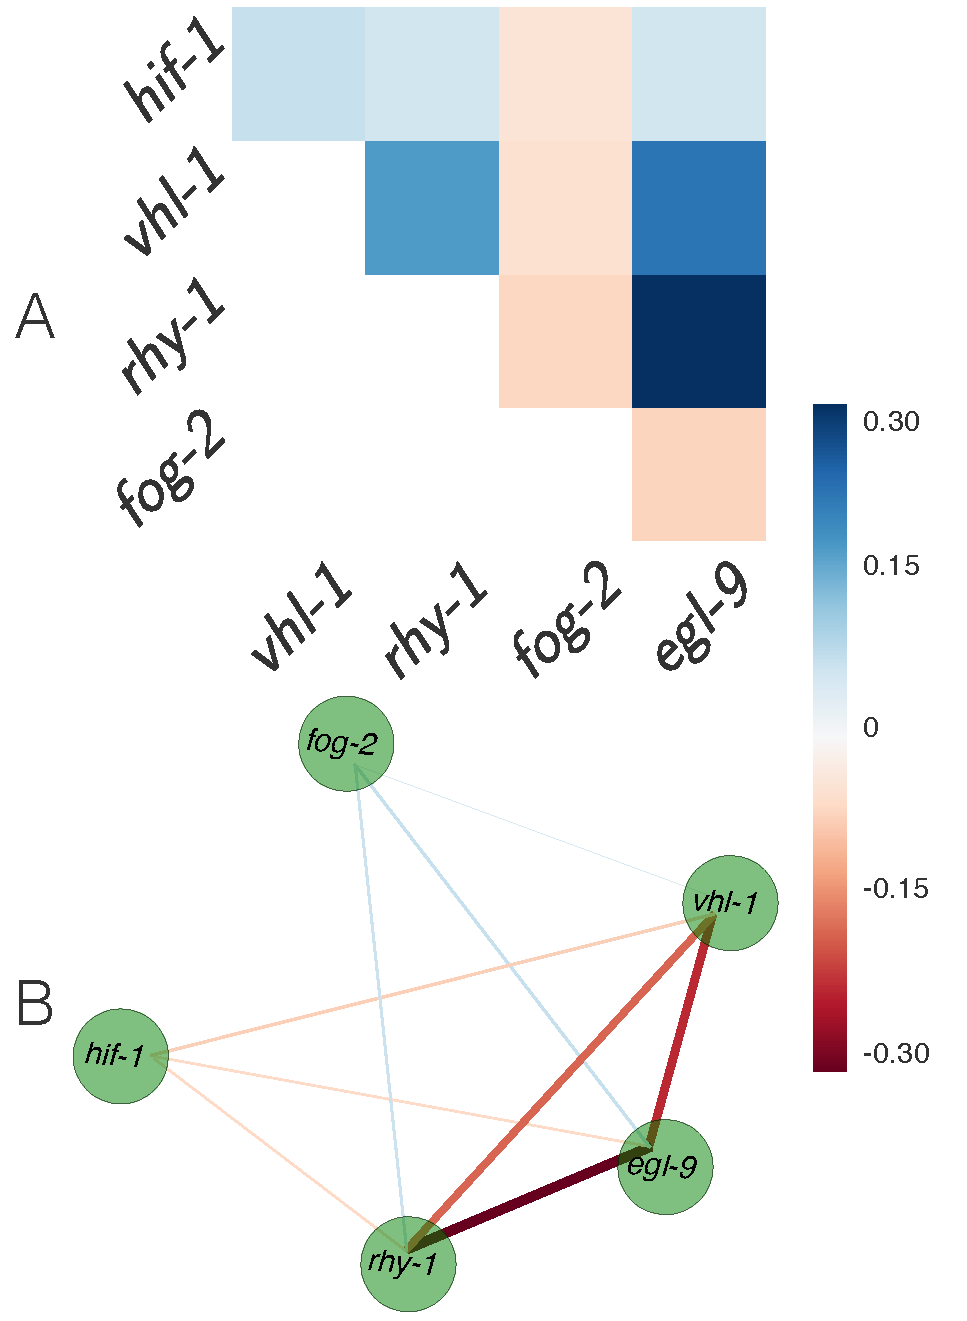
\includegraphics[width=.8\linewidth]{figs/bayesian_heat_map.pdf}
\caption{\textbf{Top}: Heatmap showing pairwise regression values between all single mutants. \textbf{Bottom}: Correlation network drawn from the diagram. Edge width is directly proportional to the regression value.}
\label{fig:heatmap}
\end{figure}

Previous work in the hypoxia pathway suggests that this pathway may have feedback loops. Using the same genetic formalism as above, we realized that interactomes due to the fine-grained nature of the data can identify two regulatory interactions if they are of opposite sign. Consider a system in which an arbitrary gene A activates a gene B, which in turn blocks a gene C. Each gene X has a specific transcriptome \emph{\{X\}}.Under this system, B and C should have transcriptomes that are negatively correlated. If C activates A, however, then knocking out B should augment expression of C, which should in turn increase expression of A.
However, knocking out C should lead to less A, which in turn will lead to less B. Under this thought experiment, suppose that we know the specific transcriptomes associated with A, B and C:\@\emph{\{A\}}, \emph{\{B\}}, \emph{\{C\}}. Then it must be the case that the genetic knockout of B must have a perturbed transcriptomes $\{A^2\}, \{B^0\}, \{C^2\}$-in other words, knocking out B increases the levels of A, which leads to an overexpression perturbation of the specific transcriptome associated with A, and so forth. On the other hand, knocking out C must lead to the perturbed transcriptomes $\{A^0\}, \{B^0\}, \{C^0\}$.
Now, if we were able to correlate each specific transcriptome between correlations, we would find that the specific transcriptomes associated with A and C are anti-correlated; whereas the specific transcriptome associated with B is correlated between both genotypes. This should lead to a characteristic \emph{X} pattern in the ranked data. Although in this particular example the cross is due to feedback loops, it is important to point out that there are other patterns that could generate these patterns.
% correlative genetics again
\begin{figure}[tbhp]
\centering
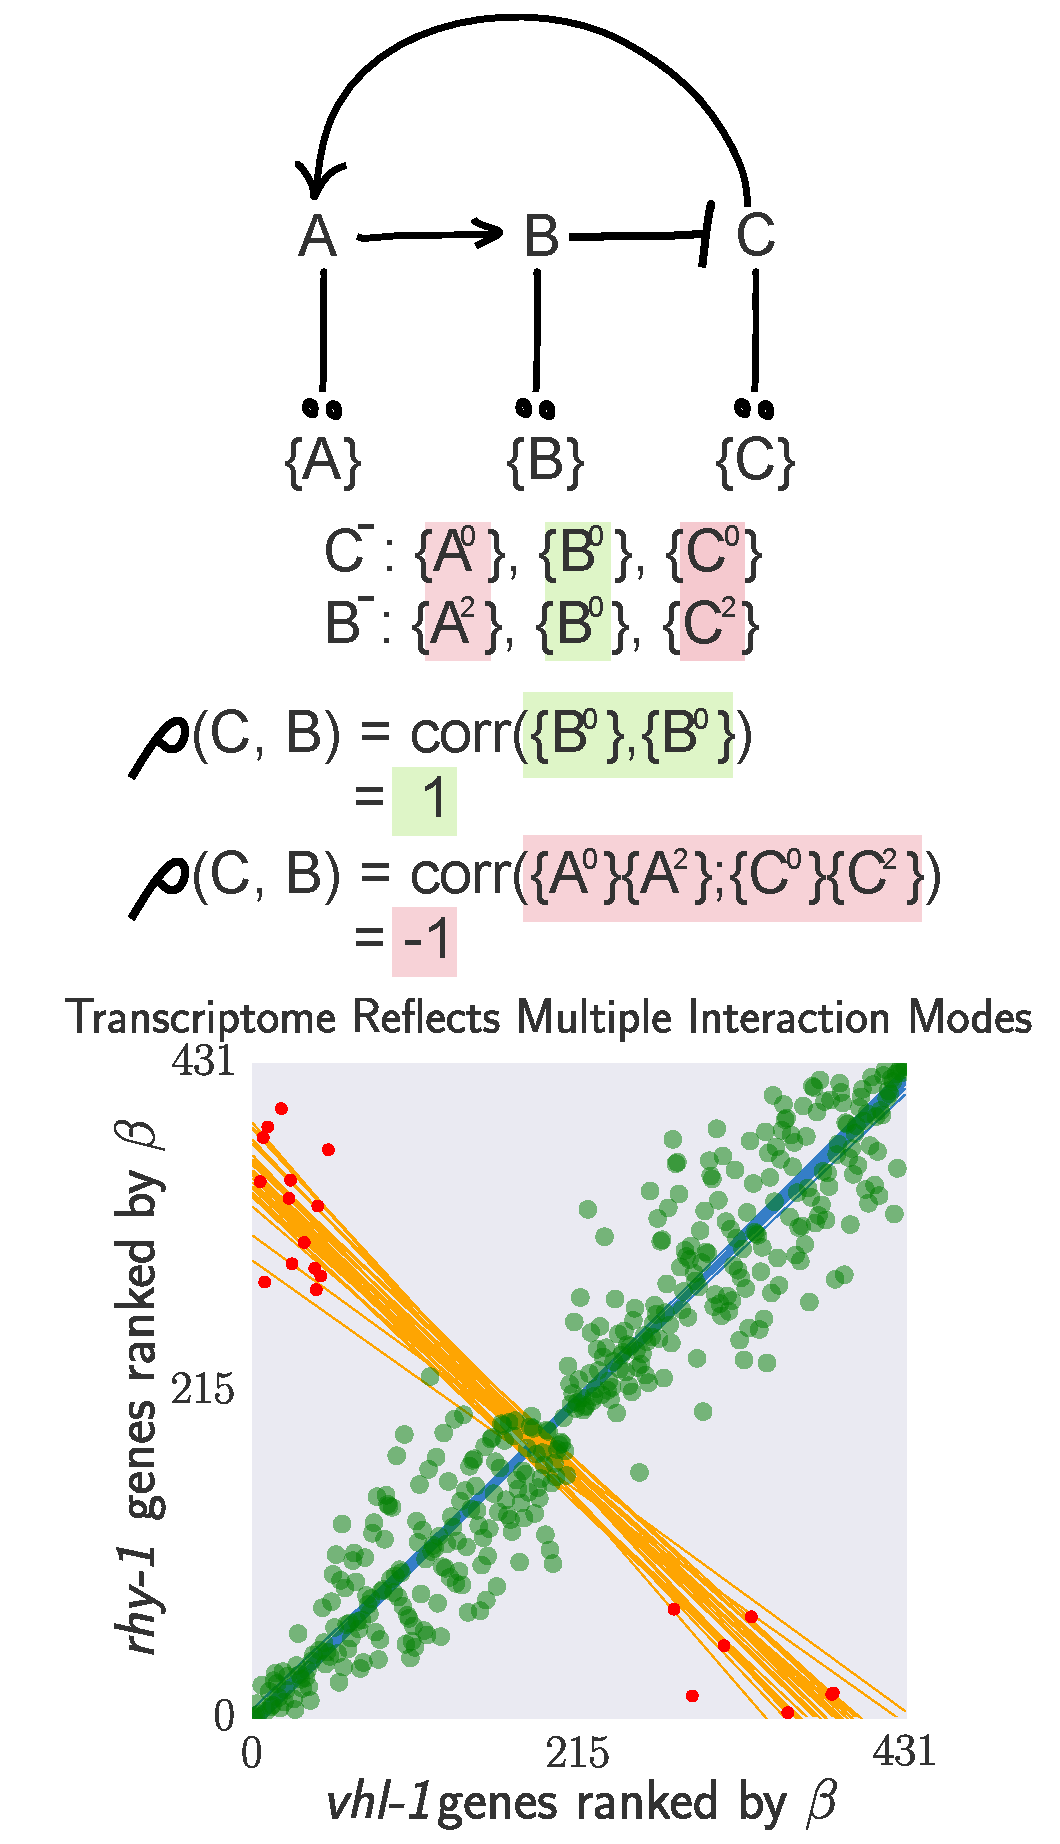
\includegraphics[width=.74\linewidth]{figs/correlative_genetics2.pdf}
\caption{\textbf{Top}: A feedback loop can generate transcriptomes that are both correlated and anti-correlated. \textbf{Bottom}: \hif{} transcriptome correlated to the \rhy{} transcriptome. Green large points are inliers to the first regression. Red small points are outliers to the first regression. Only the red small points were used for the secondary regression. Blue lines are representative samples of the primary bootstrapped regression lines. Orange lines are representative samples of the secondary bootstrapped regression lines.}
\label{fig:xpattern}
\end{figure}
 % TODO check these numbers!
We investigated whether any pairwise comparisons between our single mutants generated this cross pattern. Indeed, we found that comparing \hif{} with \rhy{}, and \hif{} with \egl{} yielded negative correlations. In fact, 8/12 possible comparisons showed a cross pattern with unweighted correlation values close to 1. However, using a hypergeometric test to examine the probability that these pairs have negative regulatory patterns, we find that the probability of negative regulation for any pair is between 4\% and 20\%.


\subsection{\emph{in silico} qPCR reveals extensive feedback in the hypoxia pathway}
\label{sub:qPCR}
We realized that our dataset enabled us to perform a sort of \emph{in silico} qPCR.\@ In order to verify the quality of our data and the veracity of \emph{in silico} qPCR, we first queried the changes in expression of \nhr{}. This particular reporter has been shown to be under direct control of \hif{}. Thus, we expected that this gene should go up in \egl{}, \rhy{} and \vhl{}, and it should be unchanged in \hif{}. The epistasis test, using the double \egl{};\hif{} double mutant should result in no change; whereas the \egl{};\vhl{} double mutant should have a similar change to the \vhl{} and the \egl{} mutants. In fact, our datasets reflected these known interactions, showing that the RNA-seq measurements can be used in a semi-quantitative fashion to perform inferences on genetic regulation.
%TODO: Verify the next paragraph is true.
Next, we decided to perform \emph{in silico} qPCR of every gene under scrutiny in order to get a clearer idea of the relationships between them (see Fig.~\ref{fig:qPCR}). We found that \rhy{} transcription levels, and to a lesser extent \egl{} levels were increased by mutations in \egl{}, \rhy{} and \vhl{}. This suggests that \hif{} is a positive regulator of \rhy{}.
Given that \rhy{} post-translationally controls \egl{}~\cite{}, it is unlikely that the increase in \egl{} is driven by the increase in \rhy{} levels. Therefore, our experiment also suggests that \hif{} is a positive regulator of \egl{}. On the other hand, we also discovered that mutation of \hif{} increased levels of \rhy{}. This suggests that \hif{} is also a negative regulator of \rhy{}. One potential mechanism through which \hif{} could be both a positive and a negative regulator would be for hydroxylation of \hif{} to change its activity. Under this mechanism, loss of \hif{} hydroxylation leads to activation of \rhy{} and \egl{} as a homeostatic mechanism, whereas excessive hydroxylation causes inhibition of these genes.

% TODO: Review the hif mRNA stuff and make sure it's good.
Whereas loss of hydroxylation seems to lead to overexpression of \rhy{} and \egl{}, there is no change in \hif{} levels. The only change in expression level of this gene occurs in the \hif{} mutant\footnote{I can't prove that this decrease in mRNA levels is not due to NMD or some other decay mechanism\ldots{}}. Therefore, we postulate that \hif{} positively autoregulates itself only in its non-hydroxylated state. The only problem with this statement is that increasing the fraction of \hif{} that is not hydroxylated by removing \egl{}, \rhy{} or \hif{} does not increase \hif{} levels. However, such steady state behavior would be expected if \hif{} had a very strong tendency to localize to its locus, in which case the \hif{} locus would be saturated even under normoxic conditions leading to its constitutive activation.

Performing the \emph{in silico} experiment with the \egl{};\vhl{} double mutant shows a similar increase in activity of the two genes in question.
This provides confirmatory evidence that \hif{} up-regulates \egl{}, but also suggests that \egl{} and \vhl{} are epistatic to one another. Such epistasis can only occur in one of two ways: Either the genes are acting linearly, or they are acting in AND gated fashion, with both genes required to mediate an effect. Similarly, the \egl{};\hif{} double mutant exhibits the same expression profile as \hif{}, which means \egl{} is an inhibitor of \hif{}.
% in silico qPCR
\begin{figure}[tbhp]
\centering
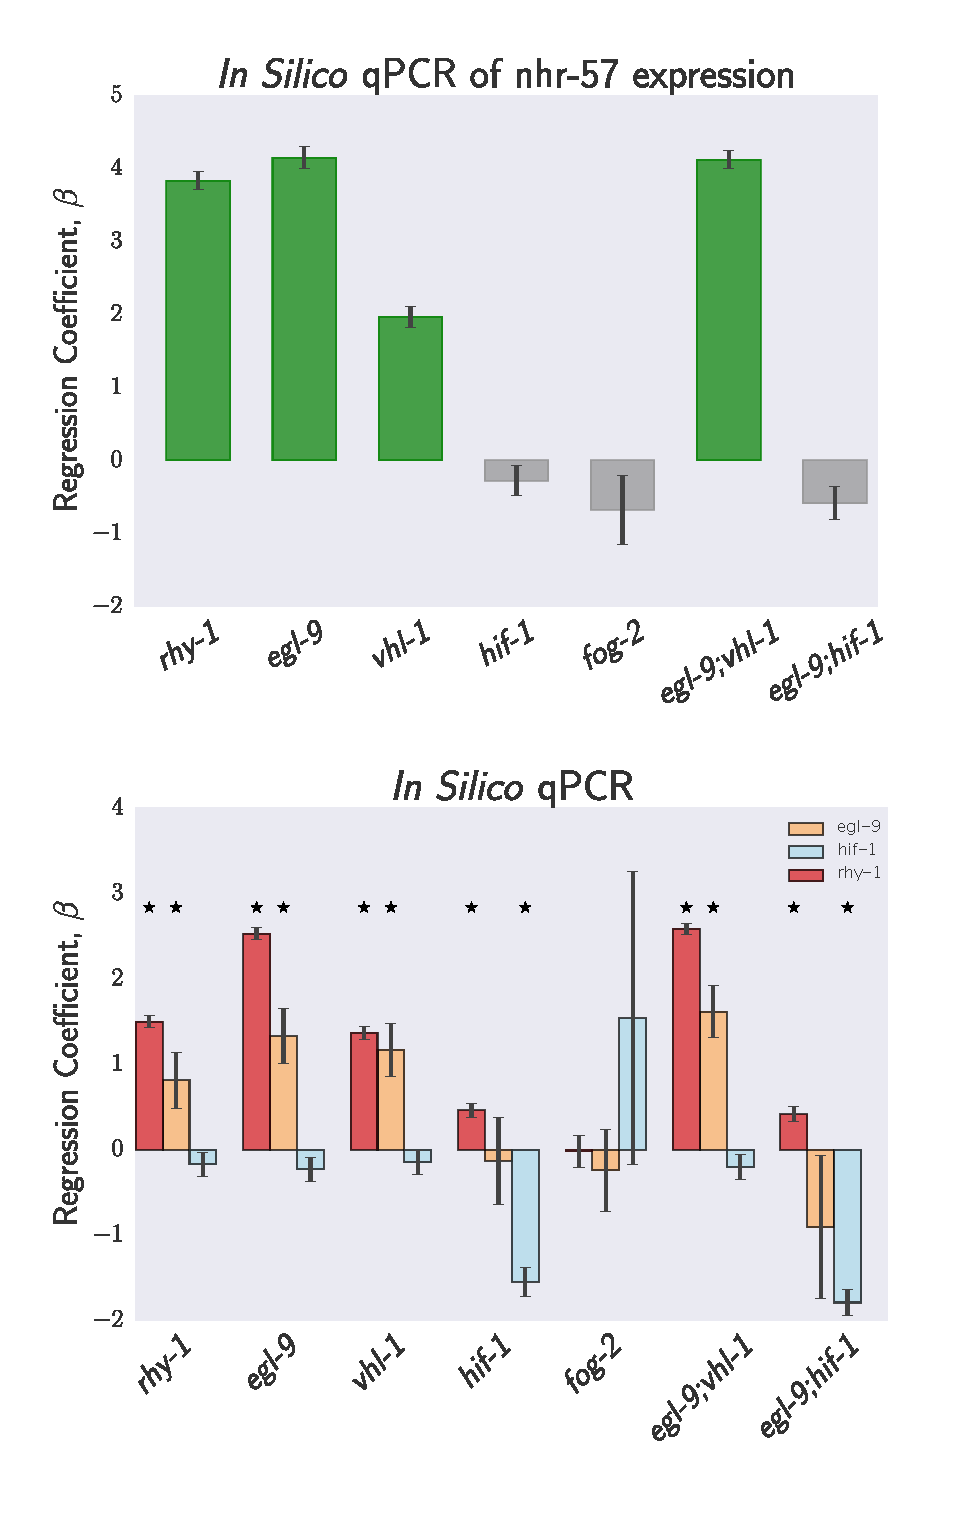
\includegraphics[width=.72\linewidth]{figs/insilico_qpcr.pdf}
\caption{\textbf{Top}: \emph{In silico} qPCR results using \nhr{} as an expression reporter. The results from the single mutants suggest that loss of \egl{} activates \nhr{} transcription, and the double mutant results show that \egl{} inhibits \hif{}; and that \egl{} and \vhl{} act in concert to inhibit \hif{}. Green bars show statistically significant increases in expression relative to wild-type. \textbf{Bottom}: \emph{In silico} qPCR of genes in the hypoxia pathway and a \fog{} control. These results suggest that \hif{} activates \rhy{}, and possibly \egl{}, when it is not hydroxylated. \hif{} also appears to autoactivate in a hydroxylation-dependent manner. Like with \nhr{}, these results support the hypothesis that \egl{} and \vhl{} together inhibit the \hif{} response.}
\label{fig:qpcr}
\end{figure}
% decorrelation
\begin{figure}[tbhp]
\centering
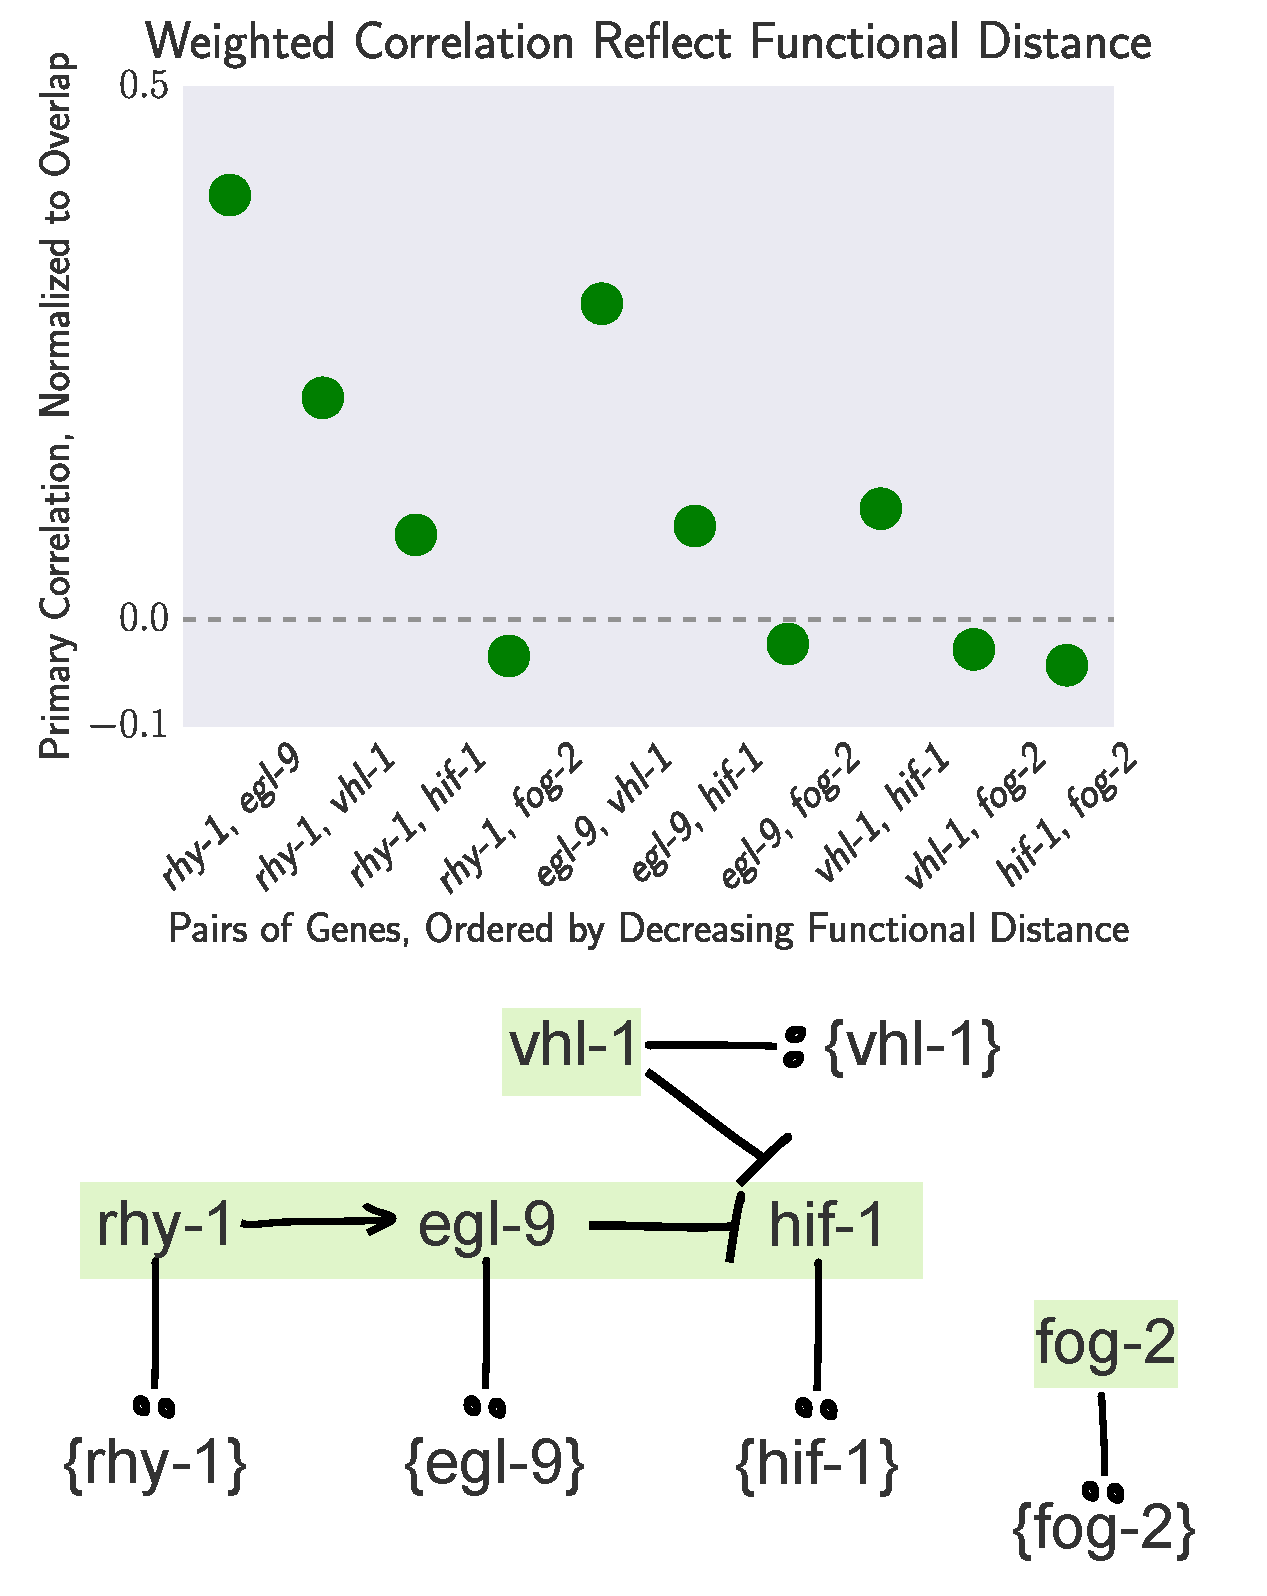
\includegraphics[width=.72\linewidth]{figs/functional_distance.pdf}
\caption{Top: Pairwise weighted correlations between transcriptomes can be used to infer functional distance between interacting genetic partners. Pairwise correlations are ordered by increasing network distance between genes. Correlations were weighted by the fraction of genes that overlapped between the two genes being compared. Notice that correlations involving the \fog{} negative control are very near zero. Bottom: Simplified schematic of the hypoxia pathway shown to illustrate functional distance between genes in the pathway.}
\label{fig:decorrelation}
\end{figure}

In summary, the \emph{in silico} qPCR results suggest that \egl{} and \vhl{} act in concert to inhibit \hif{}. Likewise, these results taken together with the transcriptome-wide cross-patterns that emerge from pairwise comparisons between genes in the hypoxia pathway suggest that there are positive and negative feedback loops feeding into \rhy{} and possibly \egl{}. These feedack loops explain why \hif{} is positively transcriptomically correlated with \egl{}--since we are observing

\subsection{Epistasis effects can be detected and quantified.}
\label{sub:Epistasis}
In order to discover whether there is evidence of \egl{} and \vhl{} acting independently of each other in our dataset, we identified the genes that were shared between each single mutant and the double mutant \egl{};\vhl{}. Under the expectation of linear/AND relationships, we would model the double mutant identically to either single mutant (the double mutant should have a slope of 1 when correlated with either single mutant). In fact, we observe that the double mutant has a worse phenotype than either single mutant (slope > 1; see Fig.~\ref{tab:double_mutant_comparison}). Indeed, we can observe that \vhl{} has a weaker effect than \egl{}, as has been previously reported~\cite{}.
% double mutant analysis
\begin{table}%[tbhp]
\centering
\caption{Response Modeling of Double Mutants to Single Mutants}
\begin{tabular}{llrr}
Double Mutant & Single Mutant & $\Delta$ & 95\% Conf. Inter.\\
\midrule
1. \egl{};\vhl{} & \egl{} & 0.18 & 0.16, 0.20\\
2. \egl{};\vhl{} & \vhl{} & 0.36 & 0.33, 0.40\\
3. \egl{};\hif{} & \egl{} & -0.38 & -0.51, -0.25\\
4. \egl{};\hif{} & \hif{} & -0.27 & -0.45, -0.09\\
\bottomrule
\end{tabular}

\addtabletext{Table showing changes between single and double mutants. $\Delta$ is the result of a weighted-linear regression (WLS) between $\beta_\mathrm{single}$ and $\beta_\mathrm{double} - \beta_\mathrm{single}$. $\Delta$ > 0 represents a more severe phenotype than the single mutant. $\Delta$ < 0 represents a suppressed phenotype relative to the single mutant. $\Delta$ = 0 is expected for linear pathways or genes that are acting in linear or AND-gated fashion. WLS were performed only on genes that were significantly altered in both single mutants and the double mutant. $1+\Delta$ is a very close approximation to the line of best fit between single mutant and double mutant.}
\label{tab:double_mutant_comparison}
\end{table}

On the other hand, comparison of the \egl{};\hif{} double mutant showed suppression of both \hif{} and \egl{} transcriptomic phenotypes. This suppression is expressed in various ways. First, the double mutant shows less statistically significantly differentially expressed genes than either single mutant. Secondly, these genes change less on average than they do in either single mutant. Whether this suppression is real is an important consideration. We conducted our experiments under normoxic conditions, where the basal levels of \hif{} are quite low. As such, the dynamic range between wild-type \hif{} and mutant \hif{} worms is low, with consequences for identification of \hif{} targets.
However, the difference between the \hif{} single and double mutant is 700 genes, and the \hif{} mutant has approximately the same number of changes as our \vhl{} mutant. Therefore, it seems unlikely that noise is entirely the reason for this suppression effect. At this point we cannot identify a molecular mechanism for this suppression.

\subsection{Transcriptomic decorrelation can be used to infer functional distance}
\label{sub:decorrelation}
We were interested in figuring out whether RNA-seq could be used to identify functional interactions within a genetic pathway. Although there is no \emph{a priori} reason why global gene expression should reflect functional interactions, we were encouraged by the strength of the unweighted correlations between genes in the hypoxia pathway, and conversely by the weak correlation of these genes with the \fog{} mutant.

We investigated the possibility that transcriptomic signals might contain relevant information about the degrees of separation by weighting the robust bayesian regression of each pairwise analysis by $N_\mathrm{Overlap}/N_{\mathrm{detected}}$. We then plotted the weighted correlation of each gene pair, ordered by increasing functional distance (see Fig.~\ref{fig:decorrelation}). In every case, we see that the weighted correlation decreases monotonically due mainly, but not exclusively, to decreasing $N_\mathrm{Overlap}$.
We believe that this result is not due to random noise or insufficiently deep sequencing. Instead, we propose a framework in which every gene is regulated by multiple different molecular species. Even in unbranched pathways, this would induce progressive decorrelation between genes.

\section*{Discussion}
% new model:
\begin{figure}[tbhp]
\centering
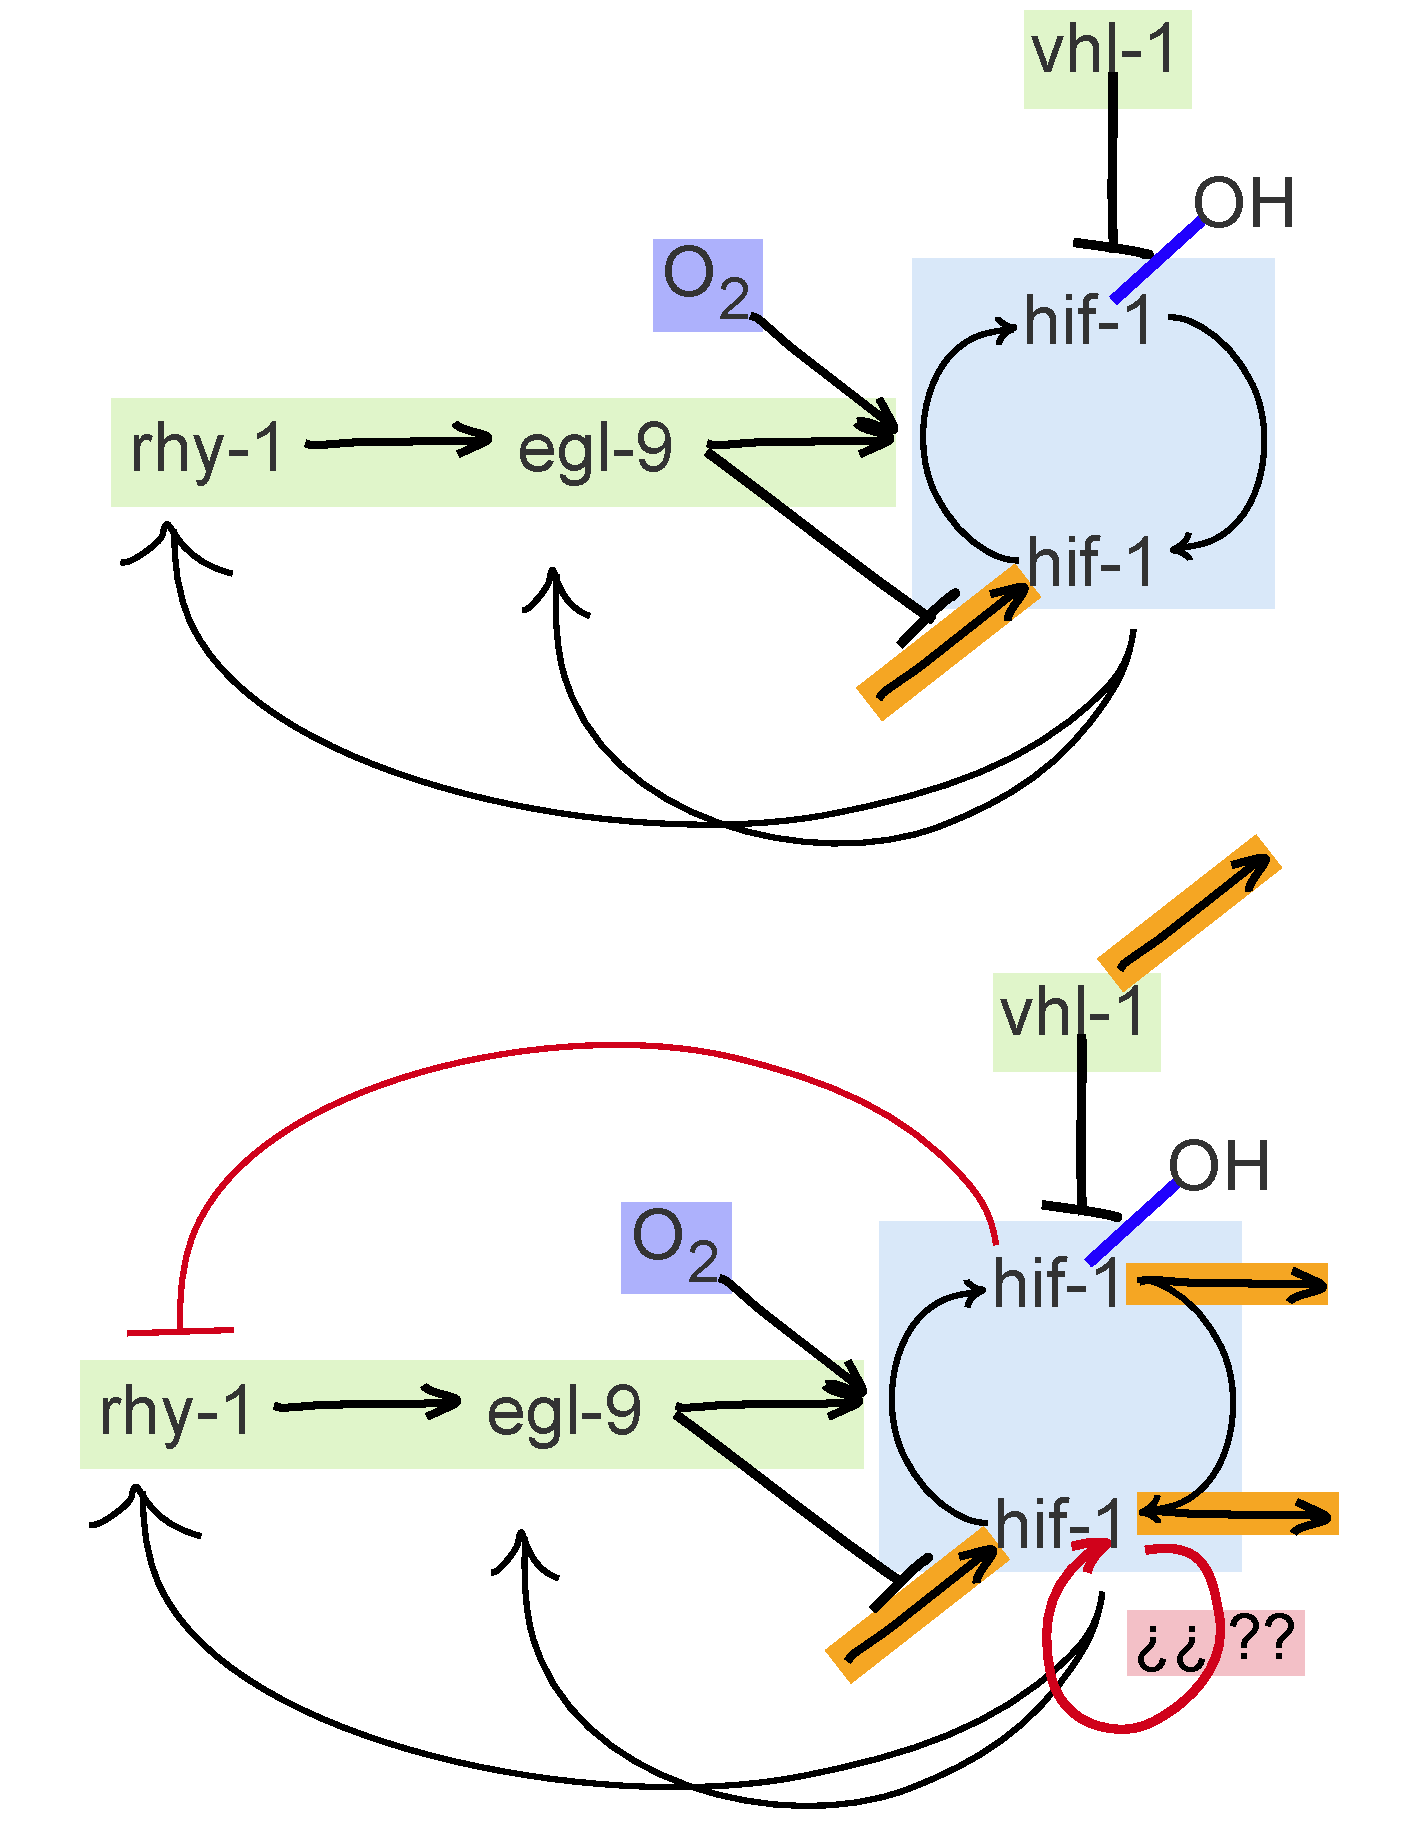
\includegraphics[width=.72\linewidth]{figs/new_model.pdf}
\caption{Top: Previous model. Bottom: Current model derived from RNA-seq data.}
\label{fig:newmodel}
\end{figure}

Previous work suggests a circuit in which \rhy{} activates \egl{} in a linear pathway~\cite{}, and \egl{} inhibits \hif{} in an oxygen-dependent manner~\cite{}. Hydroxylated \hif{} can then be degraded in a \vhl{}-dependent manner~\cite{}. There is also evidence that \egl{} and \rhy{} are in turn activated by \hif{}~\cite{}.
Finally, there is evidence that although the interaction between \egl{} and \vhl{} is important for \hif{} repression, \egl{} can also act in a non-\vhl{} dependent manner (see Fig.~\ref{fig:newmodel} top).

From our data, we were able to impute the positive regulatory relationship between \egl{} and \rhy{}. We would not have been able to infer the order of the regulation without additional information. Using clustering as a proxy for phenotype, we were able to infer the relationship between \egl{} and \hif{}. We were also able to infer a positive (linear or AND) relationship between \egl{} and \vhl{} using clustering. Alternatively, we gained the same information by performing \emph{in silico} qPCR on the genes under study. \emph{In silico} qPCR also revealed that \hif{} has two states with different activities: Non-hydroxylated \hif{} increases levels of \rhy{}, and hydroxylated \hif{} inhibits \rhy{} and possibly \egl{} as well, although the double mutant did not recapitulate that interaction. We also revealed that \hif{} is an autoregulator.

These discoveries are consistent with a homeostatic circuit. By autoregulating itself, \hif{} can mantain appropriate protein levels both in normoxic and hypoxic conditions. Inhibition of \rhy{}, and possibly of \egl{}, ensures that an appropriate equilibrium is maintained between hydroxylated and non-hydroxylated protein, which may have functional consequences for the cell if both forms are active.

In addition to these biological findings, our dataset allows us to generate predictions of genes that may be under direct \hif{} regulation. Assuming that non-hydroxylated \hif{} has different activities from hydroxylated \hif{}, we identified 5 genes that are candidates for activation by hydroxylated \hif{}. These genes have been implicated in the \cel{} immune response, or have behavioural phenotypes, underscoring the importance of \hif{} in neurobiology and immunology~\cite{}.
We also identified the gene R08E5.3 as a candidate for non-hydroxylated \hif{}. This gene, an ortholog of the human coenzyme Q5 gene, is likely essential for ubiquinone biosynthesis and as such is a primary target in respiration. We identified 167 genes that are likely to be \hif{} targets. Using a hypergeometric test, we verified that this set contains known \hif{} targets beyond random expectations (20 known targets of \hif{}, 5 genes found in our predictions, $p < 10**-6$). As expected, this gene list is enriched in genes associated with the Electron Transport Chain and metabolism in general.
Finally, we identified a set of genes 62 associated with \vhl{} in \cel{}. GO enrichment analysis using DAVID~\cite{} suggested that these genes are enriched in microtubule-associated proteins and cell-cycle regulation. Although in theory it would be possible to identify \rhy{} and \egl{} targets, these genes will be hard to discriminate from \hif{} targets because of the extensive feedback loops (indeed, many known \hif{} gene targets were excluded from our predicted dataset because of this same reason). Regardless, all predictions can be found in the SI.

We have shown that transcriptomes contain sufficient information to be used as semi-quantitative phenotypes in metazoans. These phenotypes can be interpreted globally via correlation tests, clustering or other probabilistic methods; alternatively, they can be used to query single reporter genes in a manner similar to qPCR today. Transcriptomic phenotypes have distinct advantages over physical traits. Firstly, due to their increased complexity, the genotype-phenotype mapping degeneracy ought to be greatly reduced, which facilitates predictions of genetic interaction. Secondly, genes that result in subtle or no visible traits when mutated may have strong (detectable), reproducible phenotypes at the transcriptomic level, which would make the study of small-effect genes significantly easier.
Finally, as we have shown, transcriptomic phenotypes can capture distinct interaction modes in a single experiment, making it possible to infer complex regulatory relationships between genes. With the advent of fast pseudo-alignment tools~\cite{} and ever cheaper sequencing techniques~\cite{}, biologists should consider using global transcriptomes as a tool beyond hypothesis generation or target acquisition.


\matmethods{
\subsection*{hi}
Hello
}

\showmatmethods{}% Display the Materials and Methods section

\acknow{The authors would like to acknowledge the rest of the Sternberg lab for their comments and support.}

\showacknow{} % Display the acknowledgments section

% \pnasbreak splits and balances the columns before the references.
% If you see unexpected formatting errors, try commenting out this line
% as it can run into problems with floats and footnotes on the final page.
% \pnasbreak{}

% Bibliography
\bibliography{pnas-sample}

\end{document}
